\documentclass{article}\usepackage[]{graphicx}\usepackage[]{color}
%% maxwidth is the original width if it is less than linewidth
%% otherwise use linewidth (to make sure the graphics do not exceed the margin)
\makeatletter
\def\maxwidth{ %
  \ifdim\Gin@nat@width>\linewidth
    \linewidth
  \else
    \Gin@nat@width
  \fi
}
\makeatother

\definecolor{fgcolor}{rgb}{0.345, 0.345, 0.345}
\newcommand{\hlnum}[1]{\textcolor[rgb]{0.686,0.059,0.569}{#1}}%
\newcommand{\hlstr}[1]{\textcolor[rgb]{0.192,0.494,0.8}{#1}}%
\newcommand{\hlcom}[1]{\textcolor[rgb]{0.678,0.584,0.686}{\textit{#1}}}%
\newcommand{\hlopt}[1]{\textcolor[rgb]{0,0,0}{#1}}%
\newcommand{\hlstd}[1]{\textcolor[rgb]{0.345,0.345,0.345}{#1}}%
\newcommand{\hlkwa}[1]{\textcolor[rgb]{0.161,0.373,0.58}{\textbf{#1}}}%
\newcommand{\hlkwb}[1]{\textcolor[rgb]{0.69,0.353,0.396}{#1}}%
\newcommand{\hlkwc}[1]{\textcolor[rgb]{0.333,0.667,0.333}{#1}}%
\newcommand{\hlkwd}[1]{\textcolor[rgb]{0.737,0.353,0.396}{\textbf{#1}}}%

\usepackage{framed}
\makeatletter
\newenvironment{kframe}{%
 \def\at@end@of@kframe{}%
 \ifinner\ifhmode%
  \def\at@end@of@kframe{\end{minipage}}%
  \begin{minipage}{\columnwidth}%
 \fi\fi%
 \def\FrameCommand##1{\hskip\@totalleftmargin \hskip-\fboxsep
 \colorbox{shadecolor}{##1}\hskip-\fboxsep
     % There is no \\@totalrightmargin, so:
     \hskip-\linewidth \hskip-\@totalleftmargin \hskip\columnwidth}%
 \MakeFramed {\advance\hsize-\width
   \@totalleftmargin\z@ \linewidth\hsize
   \@setminipage}}%
 {\par\unskip\endMakeFramed%
 \at@end@of@kframe}
\makeatother

\definecolor{shadecolor}{rgb}{.97, .97, .97}
\definecolor{messagecolor}{rgb}{0, 0, 0}
\definecolor{warningcolor}{rgb}{1, 0, 1}
\definecolor{errorcolor}{rgb}{1, 0, 0}
\newenvironment{knitrout}{}{} % an empty environment to be redefined in TeX

\usepackage{alltt}

\usepackage{fancyhdr} % Required for custom headers
\usepackage{lastpage} % Required to determine the last page for the footer
\usepackage{extramarks} % Required for headers and footers
\usepackage{graphicx} % Required to insert images
\usepackage{hyperref}
\usepackage{amsmath} %for binomial pdf
\usepackage{parskip} % so that there's space bw paragraphs
\usepackage{float}
\usepackage{amsfonts}

% Margins
\topmargin=-0.45in
\evensidemargin=0in
\oddsidemargin=0in
\textwidth=6.5in
\textheight=9.0in
\headsep=0.25in 

\linespread{1.1} % Line spacing

% Set up the header and footer
\pagestyle{fancy}
\lhead{STAT 532: Bayes} % Top left header
\chead{HW 3} % Top center header
\rhead{Andrea Mack} % Top right header
\lfoot{10/03/2016} % Bottom left footer
\cfoot{} % Bottom center footer
\rfoot{Page\ \thepage\ of\ \pageref{LastPage}} % Bottom right footer
\renewcommand\headrulewidth{0.4pt} % Size of the header rule
\renewcommand\footrulewidth{0.4pt} % Size of the footer rule

\setlength\parindent{0pt} % Removes all indentation from paragraphs
\setlength\parskip{0.5cm}
\restylefloat{table}

%----------------------------------------------------------------------------------------
%	DOCUMENT STRUCTURE COMMANDS
%	Skip this unless you know what you're doing
%----------------------------------------------------------------------------------------

% Header and footer for when a page split occurs within a problem environment
\newcommand{\enterProblemHeader}[1]{
\nobreak\extramarks{#1}{#1 continued on next page\ldots}\nobreak
\nobreak\extramarks{#1 (continued)}{#1 continued on next page\ldots}\nobreak
}

% Header and footer for when a page split occurs between problem environments
\newcommand{\exitProblemHeader}[1]{
\nobreak\extramarks{#1 (continued)}{#1 continued on next page\ldots}\nobreak
\nobreak\extramarks{#1}{}\nobreak
}


%----------------------------------------------------------------------------------------%
\IfFileExists{upquote.sty}{\usepackage{upquote}}{}
\begin{document}


\begin{enumerate}
\item%1 
{\it (5 points) Describe the dfferences between accept-reject sampling and importance sampling.}

Accept-reject and importance sampling are both used to estimate probability distributions and their characteristics and are especially useful when closed form solutions are not apparent. The problem arises from having a space we wish to sample from or compute characteristics of, but the space, say g(x),is not a valid pdf and so sampling from it becomes problematic. Both methods begin with sampling from a named pdf similar to g(x), say k(x). 

Accept-reject sampling only uses the subset of randomly chosen sample points under k(x) which are under g(x) and k(x). The proportion of points ``accepted" are an estimate of the proportion of the area under g(x) that is also under k(x), which can be used to estimate a sampling distribution for g(x) along with other quantities such as the area below g(x). k(x) must be greater than g(x) at all sampling points for accept-reject sampling, but not for imporatnce sampling. Importance sampling uses {\it all} the sampled observations from the chosen randomly from k(x), but weights each based on the ratio g(x)/k(x) so that the closer g(x) is to k(x), the more weight at that point. The notes did not use importance sampling as a method to estimate pdfs, but it seems taking w($x_{i}$) = $\frac{g(x_{i})}{k(x_{i})}$ a pmf can be found (or possibly estimated with a pdf with smoothing) by taking the density at each $x_{i}$ to be $\frac{w(x_{i})}{\Sigma_{i} w(x_{i})}$.

While it can be hard to estimate M, which scales a pdf to make it entirely above g(x) in accept-reject sampling, it seems that importance sampling rewards with mass similar g(x) and k(x) rather than putting more mass at peaks of g(x), but I could just not be understanding importance sampling well enough.

\begin{knitrout}
\definecolor{shadecolor}{rgb}{0.969, 0.969, 0.969}\color{fgcolor}

{\centering 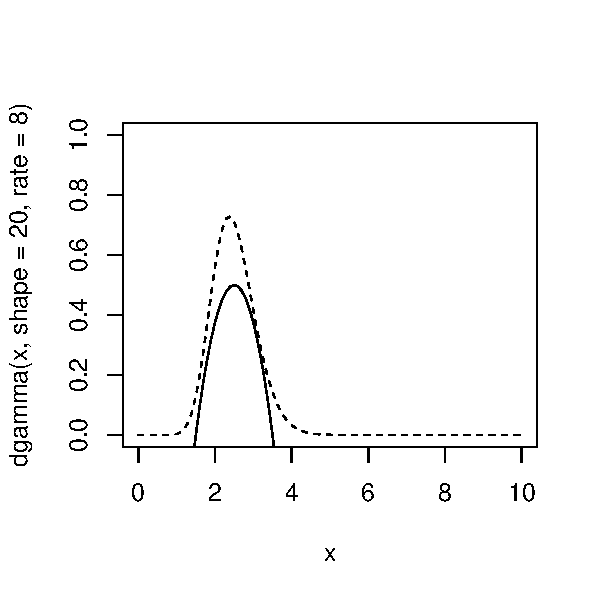
\includegraphics[width=\maxwidth]{figure/prob1-1} 

}



\end{knitrout}
\newpage

Differences:
\begin{itemize}
\item Algorithm
\item Using all sample points vs. a subset
\item Whether or not k(x) can be $\<$ g(x) at some sample points, which includes finding a constant to make this hold is necessary
\end{itemize}

\item%2
{\it (5 points) How are samples from the posterior distribution useful for inference in Bayesian statistics?}

Samples from a posterior can be used to estimate statistics such as the maximum, median, etc. of a postieror distribution and quantify the uncertainty. Sampling from the posterior using Monte Carlo methods can give estimates of the quantities with estimates of uncertainty/precision.

\item %3
{\it (5 points) Assume you are interested in obtaining a posterior predictive distribution, complete the following equation.}

$p(y^{*}|y_{1}...y_{n}) = \int p(\theta|y_{1}...y_{n})p(y^{*}|\theta) d\theta$

since 

$p(y^{*}|y_{1}...y_{n}) = \int p(y^{*},\theta|y_{1}...y_{n}) d\theta$

= $p(y^{*}|y_{1}...y_{n}) = \int p(y^{*}|\theta,y_{1}...y_{n})p(\theta|y_{1}...y_{n}) d\theta$

and since all the information contained in $y_{1}...y_{n}$ is contained in $\theta$

= $p(y^{*}|y_{1}...y_{n}) = \int p(y^{*}|\theta)p(\theta|y_{1}...y_{n}) d\theta$

= $p(y^{*}|y_{1}...y_{n}) = \int p(\theta|y_{1}...y_{n})p(y^{*}|\theta) d\theta$


\item %4
{\it (5 points) Define an improper prior and give an example of model where one might be used.}

Prior distributions do not have to be valid pdfs, as long as the posterior is valid. SAS defines an improper prior to be one where the integral over the parameter space is not finite. \url{https://support.sas.com/documentation/cdl/en/statug/63033/HTML/default/viewer.htm#statug_introbayes_sect004.htm} Before seeing this definition, I thought an improper prior was simply when the prior did not integrate to 1 over the domain, but I guess that that integral must be $\infy$ for the prior to be improper.

One way an improper prior can come about is if the input that does not follow exactly the domain of the named pdf at hand.

Making a prior improper can be used to make it less informative. We know the prior on a Poisson mean (which is also the variance) is strictly positive and that the Gamma distribution is often used as a prior on a Poisson mean, which has a domain of (0,$\infy$). If we rather used a Normal prior, which has a domain of (-$\infy$,$\infy$), we would be using an improper prior because the Poisson mean (variance) is, in reality only positive. Using the Normal may be one way of putting a less informative prior on a Poisson mean if we do not have many prior observations. An example of a Poisson random variable may be the number of bird species in a confined region, say Benton Lake area.

\item%5
{\it (20 points) Implement an accept-reject sampler to compute the area under the half-ellipse g(x) = $\sqrt$ [3(1-$\frac{x^2}{4}$)] Include your R code for full credit.}


\begin{kframe}
\begin{alltt}
\hlkwd{require}\hlstd{(truncnorm)}

\hlcom{# What is reasonable for fn_f and M}
\hlstd{fn_g} \hlkwb{<-} \hlkwa{function}\hlstd{(}\hlkwc{x}\hlstd{)\{}
  \hlstd{out} \hlkwb{<-} \hlkwd{sqrt}\hlstd{(}\hlnum{3}\hlopt{*}\hlstd{(}\hlnum{1}\hlopt{-}\hlstd{((x}\hlopt{^}\hlnum{2}\hlopt{/}\hlnum{4}\hlstd{))))}
  \hlkwd{return}\hlstd{(out)}
\hlstd{\}}

\hlstd{fn_f} \hlkwb{<-} \hlkwa{function}\hlstd{(}\hlkwc{x}\hlstd{)\{}
  \hlkwd{dtruncnorm}\hlstd{(x,}\hlkwc{a}\hlstd{=}\hlopt{-}\hlnum{1.999}\hlstd{,}\hlkwc{b}\hlstd{=}\hlnum{1.999}\hlstd{,}\hlnum{0}\hlstd{,}\hlnum{1.5}\hlstd{)}
\hlstd{\}}
\hlkwd{curve}\hlstd{(fn_g,} \hlkwc{from} \hlstd{=} \hlopt{-}\hlnum{1.999}\hlstd{,} \hlkwc{to} \hlstd{=} \hlnum{1.999}\hlstd{,}
      \hlkwc{xlim} \hlstd{=} \hlkwd{c}\hlstd{(}\hlopt{-}\hlnum{4}\hlstd{,}\hlnum{4}\hlstd{),} \hlkwc{ylim} \hlstd{=} \hlkwd{c}\hlstd{(}\hlnum{0}\hlstd{,}\hlnum{1.99}\hlstd{))}
\hlkwd{curve}\hlstd{(fn_f,} \hlkwc{add}\hlstd{=}\hlnum{TRUE}\hlstd{,} \hlkwc{lty}\hlstd{=}\hlnum{2}\hlstd{)}
\end{alltt}
\end{kframe}

{\centering 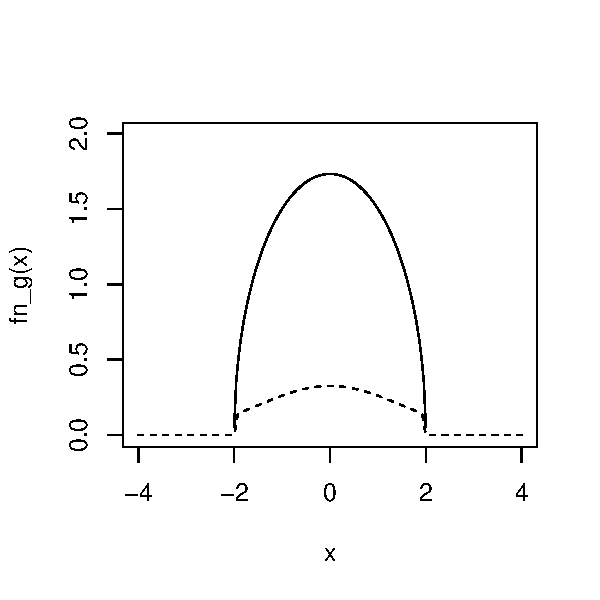
\includegraphics[width=\maxwidth]{figure/prob5-1} 

}


\begin{kframe}\begin{alltt}
\hlkwd{cat}\hlstd{(}\hlstr{"The normal(0,sd=1.5) trucated at -2 and 2 seems reasonable to 
    estimate the area of g. The next step is to find M that normalizes 
    the ratio of f and g."}\hlstd{)}
\end{alltt}
\end{kframe}The normal(0,sd=1.5) trucated at -2 and 2 seems reasonable to 
    estimate the area of g. The next step is to find M that normalizes 
    the ratio of f and g.\begin{kframe}\begin{alltt}
\hlkwd{curve}\hlstd{(}\hlkwd{fn_g}\hlstd{(x)}\hlopt{/}\hlnum{2}\hlstd{,} \hlkwc{from} \hlstd{=} \hlopt{-}\hlnum{1.999}\hlstd{,} \hlkwc{to} \hlstd{=} \hlnum{1.999}\hlstd{,}
      \hlkwc{xlim} \hlstd{=} \hlkwd{c}\hlstd{(}\hlopt{-}\hlnum{4}\hlstd{,}\hlnum{4}\hlstd{),} \hlkwc{ylim} \hlstd{=} \hlkwd{c}\hlstd{(}\hlnum{0}\hlstd{,}\hlnum{1.99}\hlstd{))}
\hlkwd{curve}\hlstd{(}\hlkwd{fn_f}\hlstd{(x)}\hlopt{*}\hlnum{3}\hlstd{,} \hlkwc{add}\hlstd{=}\hlnum{TRUE}\hlstd{,} \hlkwc{lty}\hlstd{=}\hlnum{2}\hlstd{)}
\end{alltt}
\end{kframe}

{\centering 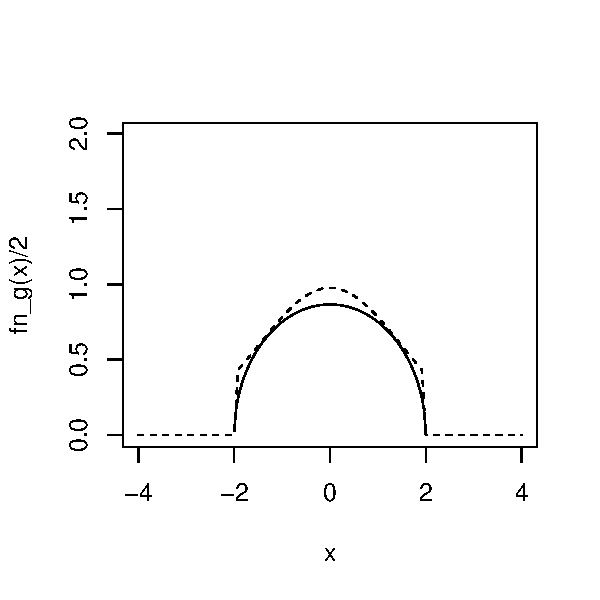
\includegraphics[width=\maxwidth]{figure/prob5-2} 

}


\begin{kframe}\begin{alltt}
\hlkwd{cat}\hlstd{(}\hlstr{"Six seems to be a reasonable constant to make f larger than g.
    Below is another method for finding the area."}\hlstd{)}
\end{alltt}
\end{kframe}Six seems to be a reasonable constant to make f larger than g.
    Below is another method for finding the area.\begin{kframe}\begin{alltt}
\hlcom{#What is reasonable for M?}

\hlcom{# Estimate the area by summing the area of squares (reimman sums), I will use the }
\hlcom{# mid point of x to estimate the height, and each bin width = 0.2}
\hlstd{s} \hlkwb{<-} \hlkwd{c}\hlstd{(}\hlkwd{seq}\hlstd{(}\hlopt{-}\hlnum{2}\hlstd{,}\hlnum{2}\hlstd{,} \hlkwc{by} \hlstd{=} \hlnum{0.2}\hlstd{))}
\hlstd{mid} \hlkwb{<-} \hlkwd{c}\hlstd{(s}\hlopt{+}\hlnum{0.1}\hlstd{)[}\hlnum{1}\hlopt{:}\hlkwd{length}\hlstd{(s)}\hlopt{-}\hlnum{1}\hlstd{]}

\hlstd{height} \hlkwb{<-} \hlkwd{fn_g}\hlstd{(mid)}
\hlstd{base} \hlkwb{<-} \hlnum{0.2}

\hlstd{area} \hlkwb{<-} \hlstd{height}\hlopt{*}\hlstd{base}
\hlstd{a} \hlkwb{<-} \hlkwd{sum}\hlstd{(area)}

\hlkwd{cat}\hlstd{(}\hlstr{"The estimated area using Reimman Sums is"}\hlstd{, a,} \hlstr{"squared units, so let M=6."}\hlstd{)}
\end{alltt}
\end{kframe}The estimated area using Reimman Sums is 5.460137 squared units, so let M=6.\begin{kframe}\begin{alltt}
\hlstd{n} \hlkwb{<-} \hlnum{10000}

\hlcom{# I am using the truncated normal distribution }
\hlcom{# with mean 0 and sd 1.5, truncated at -2 and 2}
\hlcom{# Sample randomly from the trucated distribution}
\hlstd{y} \hlkwb{<-} \hlkwd{rtruncnorm}\hlstd{(n,}\hlkwc{a}\hlstd{=}\hlopt{-}\hlnum{1.999}\hlstd{,}\hlkwc{b}\hlstd{=}\hlnum{1.999}\hlstd{,}\hlnum{0}\hlstd{,}\hlnum{1.5}\hlstd{)}
\hlcom{# summary(y)}
\hlcom{# Check, all values within -2,2}

\hlcom{# Choose M to make the trucated normal distribution }
\hlcom{# always above fn_g}
\hlcom{# requirement of accept-reject sampling}
\hlstd{M} \hlkwb{<-} \hlnum{6}

\hlkwd{set.seed}\hlstd{(}\hlnum{5323}\hlstd{)}
\hlstd{u.vals} \hlkwb{<-} \hlkwd{runif}\hlstd{(n,}\hlnum{0}\hlstd{,}\hlnum{1}\hlstd{)}
\hlcom{# Subset y to only include y such that M*fn_f(y) < fn_g(y)}
\hlstd{y.accept} \hlkwb{<-} \hlstd{y[}\hlkwd{which}\hlstd{(u.vals} \hlopt{<} \hlkwd{fn_g}\hlstd{(y)}\hlopt{/}\hlstd{(M}\hlopt{*}\hlkwd{fn_f}\hlstd{(y)))]}

\hlstd{hist_y.accept} \hlkwb{<-} \hlkwd{hist}\hlstd{(y.accept,} \hlkwc{freq} \hlstd{=} \hlnum{FALSE}\hlstd{,} \hlkwc{breaks} \hlstd{=} \hlstr{'FD'}\hlstd{,}
      \hlkwc{main} \hlstd{=} \hlstr{"Estimated pdf of g \textbackslash{}n to Sample From "}\hlstd{,} \hlkwc{xlab} \hlstd{=} \hlstr{"x"}\hlstd{)}
\end{alltt}
\end{kframe}

{\centering 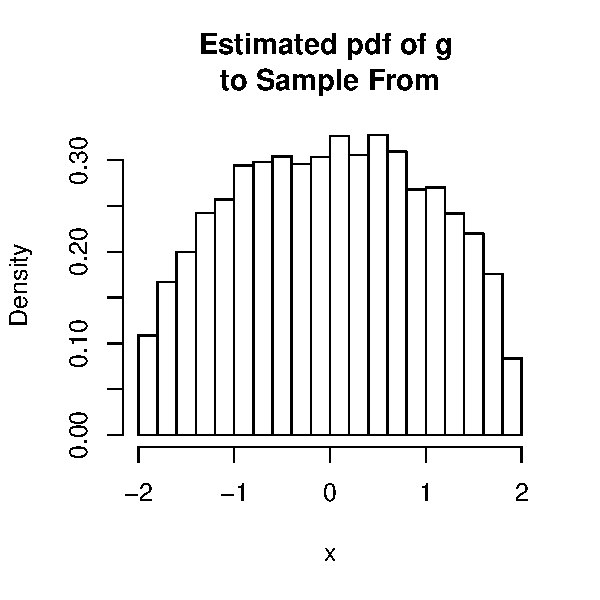
\includegraphics[width=\maxwidth]{figure/prob5-3} 

}


\begin{kframe}\begin{alltt}
\hlkwd{cat}\hlstd{(}\hlstr{"The area under the curve,"}\hlstd{,} \hlstr{"$M*f$"}\hlstd{,} \hlstr{"is 6 squared units."}\hlstd{,}
    \hlstr{"The estimated area under g using accept-reject sampling is"}\hlstd{,}
    \hlnum{6}\hlopt{*}\hlkwd{length}\hlstd{(y.accept)}\hlopt{/}\hlkwd{length}\hlstd{(y),} \hlstr{"squared units."}\hlstd{)}
\end{alltt}
\end{kframe}The area under the curve, $M*f$ is 6 squared units. The estimated area under g using accept-reject sampling is 5.4048 squared units.

\item%6 

Problem 6 is attached.

\item%7

\begin{enumerate}
\item%7a
{\it (5 points) How would you go about addressing the researcher's questions in a classical
framework? Would you be able to compute these probabilities?}

Under a classical framework, I would have to know the true pdf and its associated parameters to compute these probabilities. The normal pdf may be reasonable, but I would have to know or find a good resource for the parameters associated with the normal distribution.

If it was reasonable that the mean snowfall at Graf Park did not depend on the mean snow fall at Cherry River, then I would use the bivariate normal distribution for the joint pdf. 











I would compute these probabilities using the probability functions in R.

\item%7b
{\it (5 points) How would you address the researcher's questions in a Bayesian framework? Can you compute these probabilities?}

In a Bayesian framework I would compute each of the three posterior pdfs, and ideally each would be a conjugate pair of a named distribution, so we could again use the probability functions in R.

Realistically, for example, with $p(\theta|y_{1},...,y_{n}) = \int_{\sigma^{2}}p(y_{1},...,y_{n}|\theta,\sigma^{2})*p(\theta|\sigma^{2})*p(\sigma^{2}) d\sigma^{2}$ with

$y_{1},...,y_{n}|\theta,\sigma^{2} \sim$ N($\theta,\sigma^{2})$

$\theta|\sigma^{2} \sim$ N($\mu_{o},\sigma^2/k_{o}$)

$\sigma^{2} \sim$ INVGAM($\frac{\nu_{o}}{2},\frac{\nu_{o}*\sigma_{o}^2}{2}$)

finding a closed form solution is not feasible and the posteriors have to be estimated using Monte Carlo procedures.

\item%7c
Kenny says that choosing $\kappa_{o}$ larger means we have more information about $\theta$, or a stronger prior distribution on $\theta$ whereas choosing a larger $\nu_{o}$ means we have more information about $\sigma^{2}$, meaning a stronger prior on $\sigma^{2}$. In practice, I would plot several priors with different $\kappa_{o}$ and $\nu_{o}$ values and ask the researcher which he thought to most resemble the true prior distributions to find estimates of these parameters.

I estimated $\theta$ or the mean, using a website, so I will choose $\kappa_{o}$ to be larger, say 50. I have no idea about what $\sigma^{2}$ should be, so I will choose $\nu_{o}$ = 1. I choose $\sigma^{2}$ = $10^{2}$ = 100 because we expect 95\% of data to lie within about two standard deviations of the mean and if I am using about 231.1 cm as the true mean snowfall, I would expect most years the mean snowfall be be between 210 and 250.

\newpage

P( $\theta_{gp}$ )

{\centering 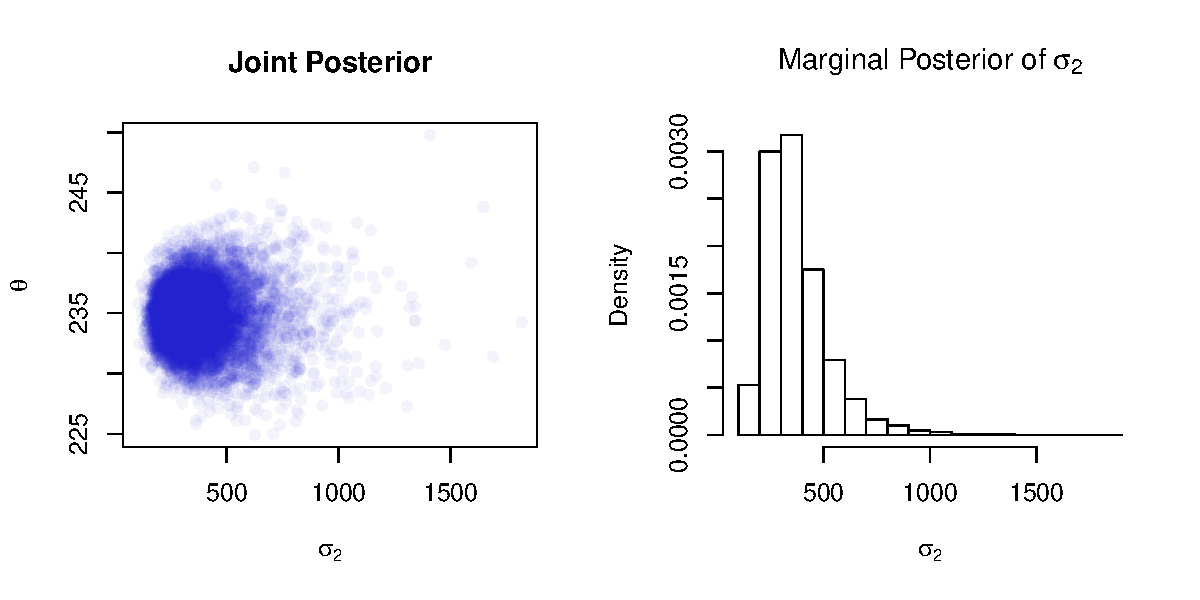
\includegraphics[width=\maxwidth]{figure/prob7c1-1} 

}


P( $\theta_{gp}$ $>$ 250 ) = 0

{\centering 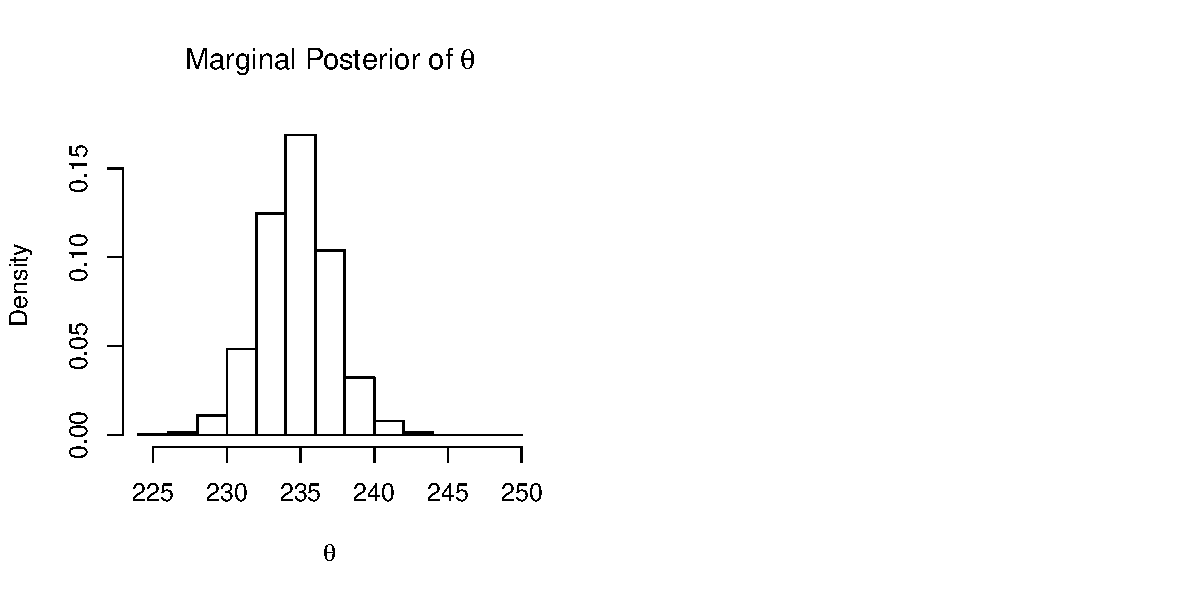
\includegraphics[width=\maxwidth]{figure/prob7c1-2} 

}



\newpage

P( $\theta_{cr}$ )

{\centering 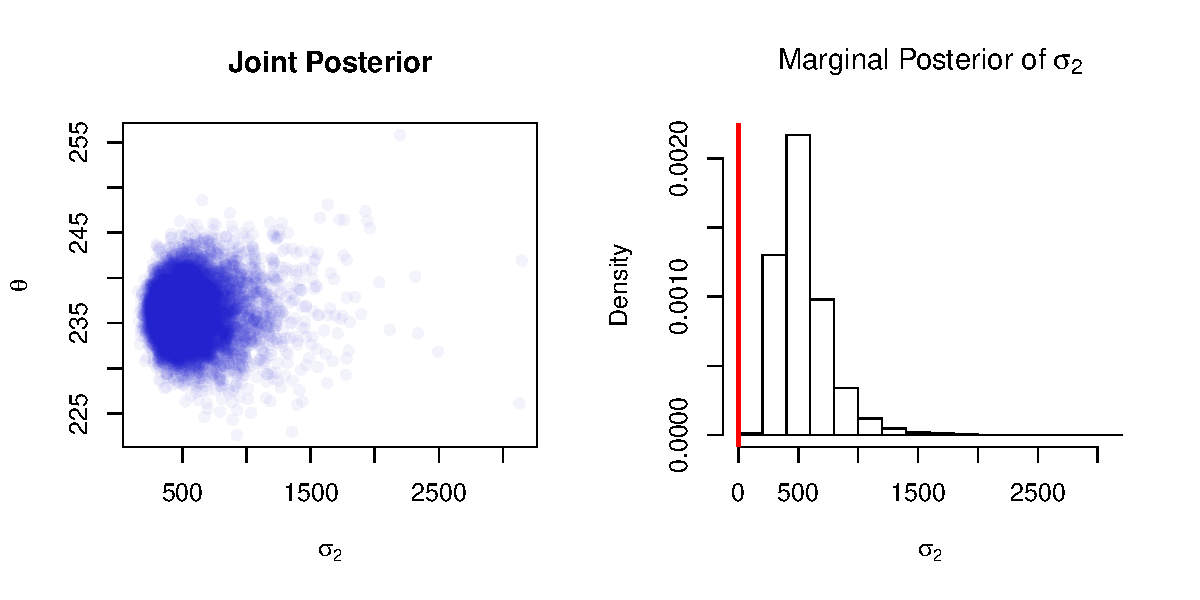
\includegraphics[width=\maxwidth]{figure/prob7c2-1} 

}


P( $\theta_{cr}$ $>$ 250 ) = 1e-04

{\centering 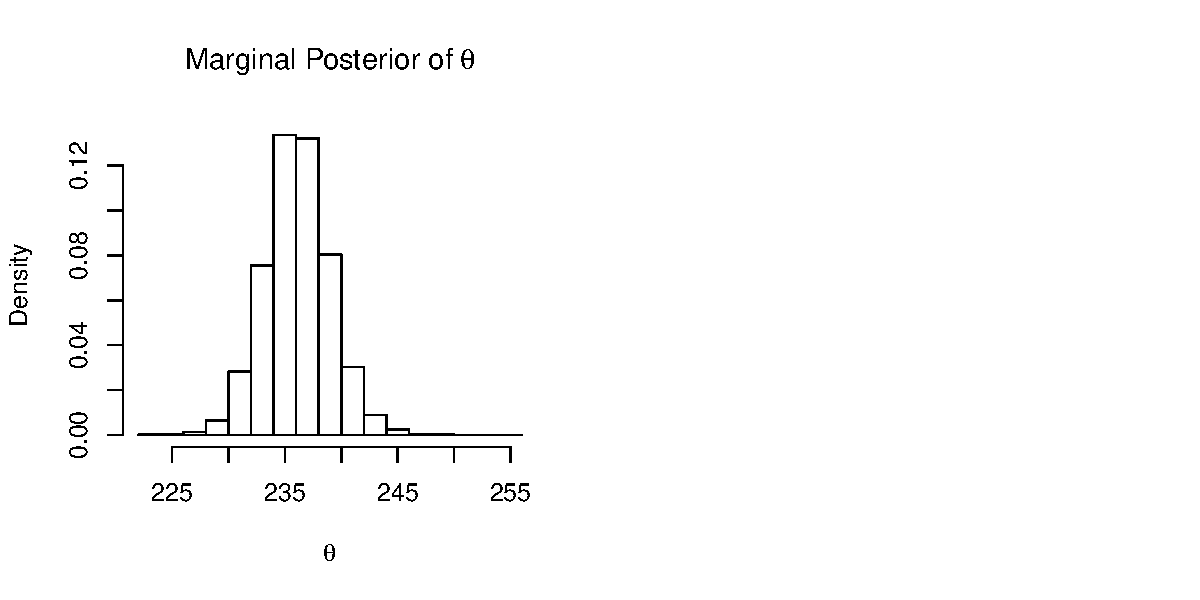
\includegraphics[width=\maxwidth]{figure/prob7c2-2} 

}




P( $\theta_{cr}$ , $\theta_{gp}$ )If we can assume $\theta_{cr}$ and $\theta_{gp}$ are indepdendent,
    which would mean that knowing the mean snowfall at Cherry River does not tell us
    anything about the snowfall at Graf Park, then P( $\theta_{cr}$ , $\theta_{gp}$ ) = P( $\theta_{cr}$ ) $\times$ P( $\theta_{cr}$ ). This does not seem
    reasonable, but is what I will assume for this problem. Then $\theta_{cr} - $\theta_{gp}$ $\sim$ BIVNORM( 0 $\frac{2*\sigma^{2}_{i}}{k_{n}}$ ) where $\sigma^{2}_{i}$ is generated randomly from an inverse gamma distribution. Note that
    in addition to assuming independence, I also assumed the two parameters have a common mean
    and common variance.

{\centering 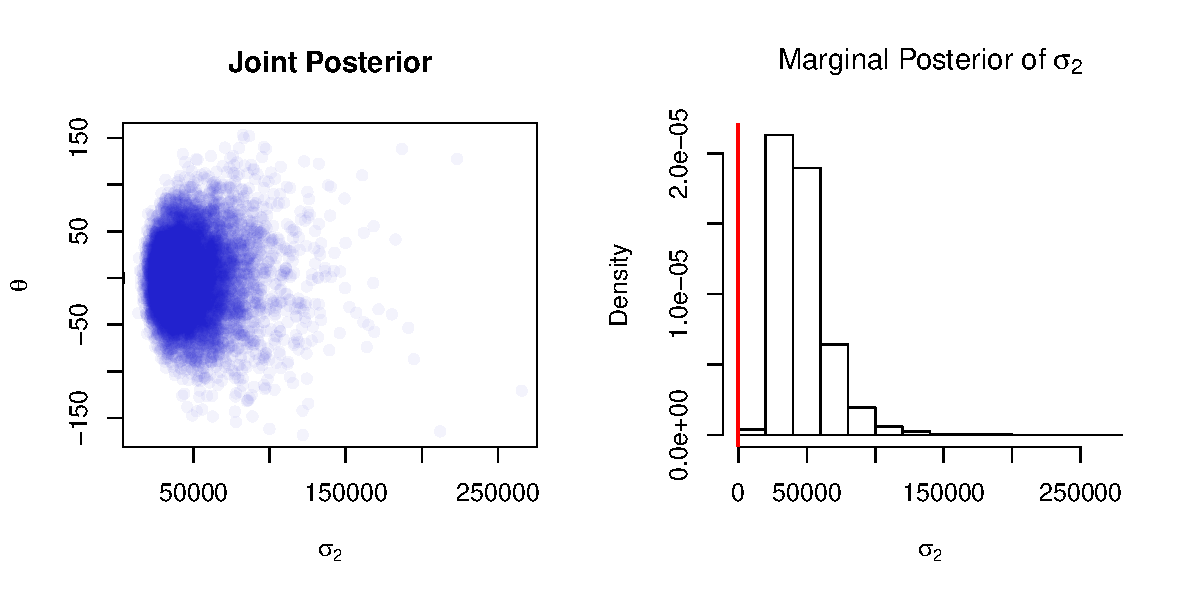
\includegraphics[width=\maxwidth]{figure/prob7c3-1} 

}


P( $\theta_{cr}$ - $\theta_{gp}$ $>$ 0 ) = 0.4998

{\centering 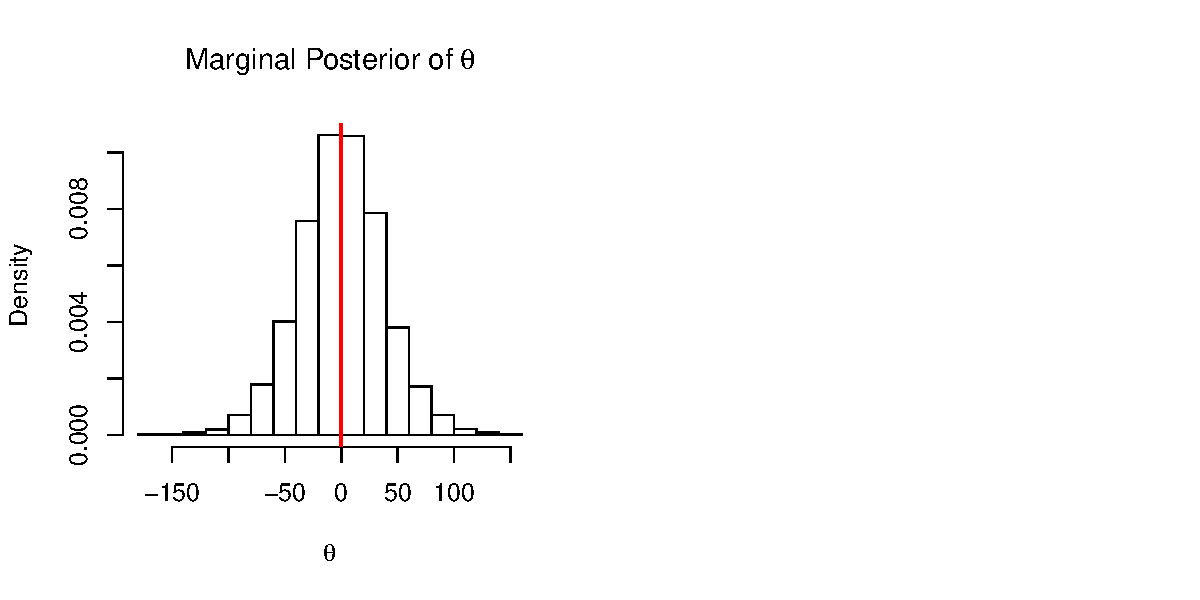
\includegraphics[width=\maxwidth]{figure/prob7c3-2} 

}




Thoughts: I probably should not have set the prior to having a low chance of being above 250 in the prior, but seeing that I put less strength on the prior using $\nu_{o}$ = 1, I did not think it would have influenced the posterior that much.

\end{enumerate}
\end{enumerate}

\end{document}
